\documentclass[12pt]{article}
\usepackage[english]{babel}
\usepackage[letterpaper,top=2cm,bottom=2cm,left=3cm,right=3cm,marginparwidth=1.75cm]{geometry}
\usepackage{amsmath}
\usepackage{graphicx}
\usepackage{gensymb}
\DeclareMathOperator{\erf}{erf}
\DeclareMathOperator{\probit}{probit}
\title{STAT-UB 103 Homework 6}
\author{Ishan Pranav}
\date{March 21, 2023}
\renewcommand{\thesubsection}{\thesection.\alph{subsection}}
\renewcommand{\theenumi}{\alph{enumi}}
\newcommand{\degreeF}{\degree F}
\begin{document}
\maketitle
\section{A recent survey}
Let it be assumed each instance of a credit-card balance paid in full is completely independent of all other instances. Each person either pays or does not pay their credit card bill in full. Since there are a fixed number of independent binary trials ($n$), each with a known probability of success ($p$), the probability that the number of bills paid ($X$) is equal to a given value ($k$) can be modeled with a binomial random variable.

\[n=400.\]

\[p\approx 0.30.\]

\[P(X=k)=p_k={\binom{n}{k}}p^k(1-p)^{n-k}.\]

\begin{enumerate}
\item\[P(X\geq k)=\sum^{n}_{i=k}{p_i}=\sum^{n}_{i=k}{{\binom{n}{i}}p^i(1-p)^{n-i}}.\]

\[P(X\geq 110)\approx\sum^{400}_{i=110}{{\binom{400}{i}}(0.30)^i(0.70)^{400-i}}\approx 0.87.\]

\item\[P(X<k)=\sum^{k-1}_{i=0}{\binom{n}{i}p^i(1-p)^{n-i}}.\]

\begin{align*}
P(125\leq X<140)
&=P(X<140)-P(X<125)\\
&=P(X<140)-P(X<125)\\
&\approx\left[\sum^{139}_{i=0}{\binom{400}{i}(0.30)^i(0.70)^{400-i}}\right]-\left[\sum^{124}_{i=0}{\binom{400}{i}(0.30)^i(0.70)^{400-i}}\right]\\
&\approx 0.29.
\end{align*}
\end{enumerate}
\section{The daily returns on a portfolio}
Let $X$ represent the daily returns on a portfolio, $\mu_X$ represent the mean daily return, and $\sigma_X$ represent the standard deviation of daily returns.

\[\mu_X\approx 0.001.\]

\[\sigma_X\approx 0.002.\]
\begin{enumerate}
\item The probability that the number of positive-return days of the next 100 days ($Y$) greater than or to a given value ($k$) can be modeled with a binomial random variable.

\[P(Y\geq k)=\sum^{n}_{i=k}{p_i}=\sum^{n}_{i=k}{{\binom{n}{i}}p^i(1-p)^{n-i}}.\]

\[n=100.\]

\[p\approx P(X>0)\approx 1-P(X\leq 0).\]

The probability of a positive portfolio return on a given day ($p$) is dependent on the return itself, which can be modeled with a Gaussian random variable.

\[z_x=\frac{x-\mu_X}{\sigma_X}.\]

\[z_0\approx\frac{0-0.001}{0.002}\approx -0.5.\]

\[\varphi(z)=\frac{e^{-\frac{z^2}{2}}}{\sqrt{2\pi}}.\]

\[\Phi(x)=\int^x_{-\infty}{\varphi(t)\,\mathrm{d}t}=\frac{1}{\sqrt{2\pi}}\int^x_{-\infty}{e^{-\frac{t^2}{2}}\,\mathrm{d}t}.\]

\[P(z\leq x)=\Phi(x).\]

\[p\approx 1-P(z\leq -0.5)\approx 1-\Phi(-0.5)\approx 0.7.\]

\[P(Y\geq 60)\approx\sum^{100}_{i=60}{{\binom{100}{i}}(0.7)^i(0.3)^{100-i}}\approx1.\]

\item The probability that the average return for the portfolio over the next 100 days ($\bar{X}$) exceeds 0.0015 follows from the Central Limit Theorem.

\[\mu_{\bar{X}}=\mu_X\approx 0.001.\]

\[\sigma_{\bar{X}}=\frac{\sigma_X}{\sqrt{n}}\approx\frac{0.002}{\sqrt{100}}\approx 0.0002.\]

\begin{align*}
P(\bar{X}>0.0015)
&=P\left(z>\frac{0.0015-\mu_X}{\sigma_{\bar{X}}}\right)\\
&\approx P\left(z>\frac{0.0015-0.001}{0.0002}\right)\\
&\approx 1-P(z\leq 2.5)\\
&\approx 1-\Phi(2.5)\\
&\approx 0.006.
\end{align*}
\end{enumerate}
\section{In May 1983}
Let it be assumed each instance of a defective smoke detector is completely independent of all other instances. Each smoke detector is either defective or not effective. Since there are a fixed number of independent binary trials ($n$), each with a known probability of success ($p$), the probability that the number of defective smoke detectors discovered ($X$) is less than or equal to a given value ($k$) can be modeled with a binomial random variable.

\[P(X\leq k)=\sum^{k}_{i=0}{\binom{n}{i}p^i(1-p)^{n-i}}.\]

The null hypothesis ($H_0$) is the Commission's suggestion that 40 percent of Honeywell smoke detectors are defective.

\[n=2000.\]

\[H_0: p=0.4.\]

\[P(X\leq 4\,|\,H_0)=\sum^{4}_{i=0}{\binom{2000}{i}(0.4)^i(0.6)^{2000-i}}\approx 2\times 10^{-433}.\]
\section{Game}
Let it be assumed each coin flip is completely independent of all other coin flips. Each coin lands on either the obverse side or the reverse side. Since there are a fixed number of independent binary trials ($n$), each with a known probability of success ($p$), and because the number of obverse coins is material ($np\geq 10$) and the number of reverse coins is material ($(n)(1-p)\geq 10$), the number of obverse coins ($X$) can be modeled with a binomial random variable, and it is appropriate to use the normal approximation to the binomial distribution.

\[n=100.\]

\[p=0.5.\]

\[np=50\geq 10.\]

\[(n)(1-p)=50\geq 10.\]

Let $c$ represent the compensation received for a given number of obverse coins ($x$).

\begin{equation*}
c_x=\begin{cases}
    \$20,&x\geq 60\\
    -\$1,&x<60.
\end{cases}
\end{equation*}
\begin{align*}
P(X\geq 60)
&=P\left(z\geq\frac{60-\mu_X}{\sigma_X}\right)\\
&=P\left(z\geq\frac{60-np}{\sqrt{(n)(p)(1-p)}}\right)\\
&\approx 1-P\left(z<\frac{59.5-np}{\sqrt{(n)(p)(1-p)}}\right)\\
&\approx 1-P(z\leq 1.9)\\
&\approx 1-\Phi(1.9)\\
&\approx 0.02871\dots
\end{align*}
\begin{align*}
\mu_C
&=\sum{cp_{c}}\\
&=\$20\times P(X\geq 60)-\$1\times P(X<60)\\
&=\$20\times P(X\geq 60)-\$1\times(1-P(X\geq 60))\\
&=\$21\times P(X\geq 60)-\$1\\
&\approx-\$0.3970\dots\\
&\approx-\$0.40.
\end{align*}
The expected loss is \$0.40. This is not a good game to play.
\section{Data on body temperatures}
The 95-percent confidence interval for $\mu$ is (98.1220, 98.3765). Yes, the results of the confidence interval are surprising, since the confidence interval does not contain the assumed population mean temperature of 98.6\degreeF.
\begin{figure}[h]
\begin{center}
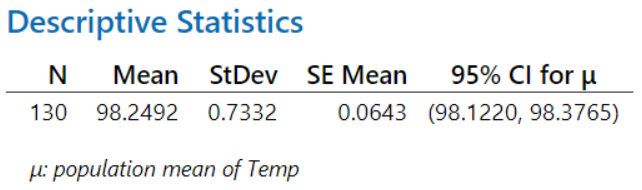
\includegraphics[width=3in]{images/temperature-confidence-interval.png}
\end{center}
\caption{Ninety-five-percent confidence interval for temperature.}
\end{figure}
\end{document}